\subsection{RAT-SQL} \label{sec:ratsql}

RAT-SQL, or Relation-Aware Schema Encoding and Linking\cite{wang_rat_sql_2021}, is a method used in text-to-SQL parsers to improve the accuracy of SQL generation. A significant issue in transforming natural language queries into SQL queries is generalizing them to unfamiliar database schemas. As part of the generalization process, it is crucial to represent database relations comprehensibly and to model the alignment between pertinent database columns in the query. Within a Text-to-SQL encoder, the proposed framework employs a relation-aware self-attention mechanism to encode schemas, illustrate features, and connect schemas.

% \begin{figure}[htb]
%     \centering
%     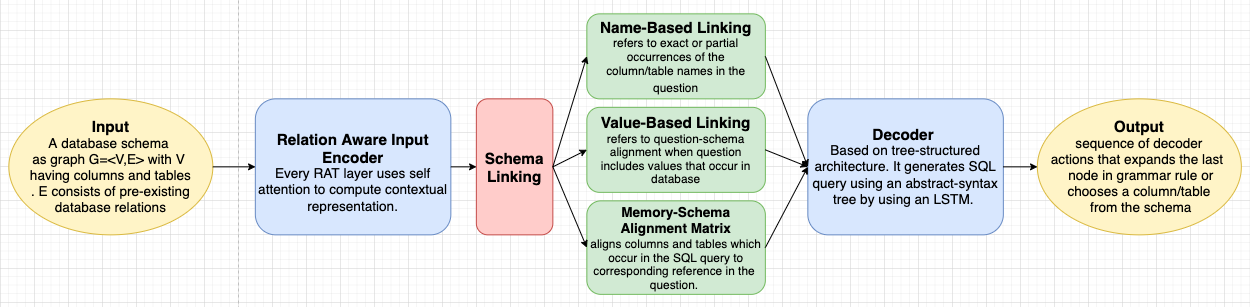
\includegraphics[width=0.8\textwidth]{pics/RAT-SQL/flow.png}
%     \caption{A flow chart of RAT-SQL's encoder-decoder structure}
%     \label{fig:RAT-SQL-flow}
% \end{figure}

On the SPIDER dataset, RAT-SQL achieved a 57.2\% accuracy score, which is 8.7\% higher than the accuracy of prior benchmark models. Combining BERT with RAT-SQL further increased the accuracy to 65.6\%.


% \begin{figure}[htb]
%     \centering
%     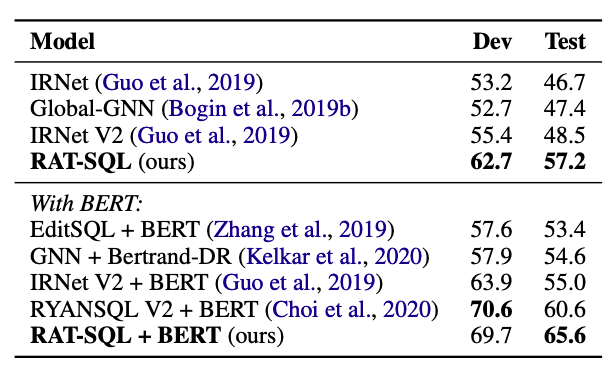
\includegraphics[width=0.4\textwidth]{pics/RAT-SQL/Accuracy.png}
%     \caption{Accuracy on the Spider development and test sets, compared to the other approaches at the top of the dataset leaderboard as of May 1st, 2020 from \cite{wang_rat_sql_2021}}
%     \label{fig:RAT-SQL-Accuracy}
% \end{figure}
% \begin{figure}[htb]
%     \centering
%     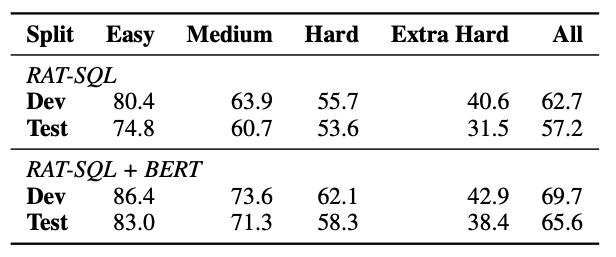
\includegraphics[width=0.4\textwidth]{pics/RAT-SQL/Accuracy2.png}
%     \caption{Accuracy on the Spider development and test sets, by difficulty from \cite{wang_rat_sql_2021}}
%     \label{fig:RAT-SQL-Accuracy2}
% \end{figure}